\documentclass[a4paper,oneside]{article}
\usepackage{noweb}
% Needed to relax penalty for breaking code chunks across pages, otherwise 
% there might be a lot of space following a code chunk.
\def\nwendcode{\endtrivlist \endgroup}
\let\nwdocspar=\smallbreak

\usepackage[hyphens]{url}
\usepackage{hyperref}
\usepackage{authblk}

\usepackage[utf8]{inputenc}
\usepackage[T1]{fontenc}
\usepackage[swedish,british]{babel}
\usepackage{booktabs}

\usepackage[natbib,style=alphabetic,maxbibnames=99]{biblatex}
\addbibresource{bibliography.bib}

\usepackage[inline]{enumitem}
\setlist[enumerate]{label=(\arabic*)}

\usepackage[all]{foreign}
\renewcommand{\foreignfullfont}{}
\renewcommand{\foreignabbrfont}{}

%\usepackage{newclude}
\usepackage{import}

\usepackage[strict]{csquotes}
\usepackage[single]{acro}

\usepackage{subcaption}

\usepackage[noend]{algpseudocode}
\usepackage{xparse}

\let\email\texttt

\usepackage[outputdir=ltxobj]{minted}
\setminted{autogobble,linenos}

\usepackage{pythontex}
\setpythontexoutputdir{.}
\setpythontexworkingdir{..}

\usepackage{fancyvrb}

\usepackage{amsmath}
\usepackage{amssymb}
\usepackage{mathtools}
\usepackage{amsthm}
\usepackage{thmtools}
\usepackage[unq]{unique}
\DeclareMathOperator{\powerset}{\mathcal{P}}

\usepackage[binary-units]{siunitx}

\usepackage{pgf}

\usepackage[capitalize]{cleveref}
\crefalias{question}{item}
\crefname{question}{question}{questions}
\Crefname{question}{Question}{Questions}
\creflabelformat{question}{#2\textup{#1}#3}



\title{%
  \texttt{weblogin}: Automates logging into web UIs to access unofficial APIs
}
\author{%
  Daniel Bosk
}
\affil{%
  KTH EECS\\
  \texttt{dbosk@kth.se}
}

\begin{document}
\maketitle
\begin{abstract}
  We provide a Python package that can be used to automate logging in to web UIs 
to access the APIs that the UIs are using.

\end{abstract}

\clearpage
\vspace*{\fill}
\VerbatimInput{../LICENSE}
\clearpage

\clearpage

\tableofcontents
\clearpage

\section{Introduction}

We want to use APIs from web UIs that require login.
What we want to do is to set up a session, login and then use the API of the 
page.
The reason we want to do this is to use existing APIs.
For instance, the user group management service at KTH, see \cref{UGEditor}.
We can then use the service, track the requests in the browser's developer 
tools.
Then we can simply make the same requests from Python.

\begin{figure}
  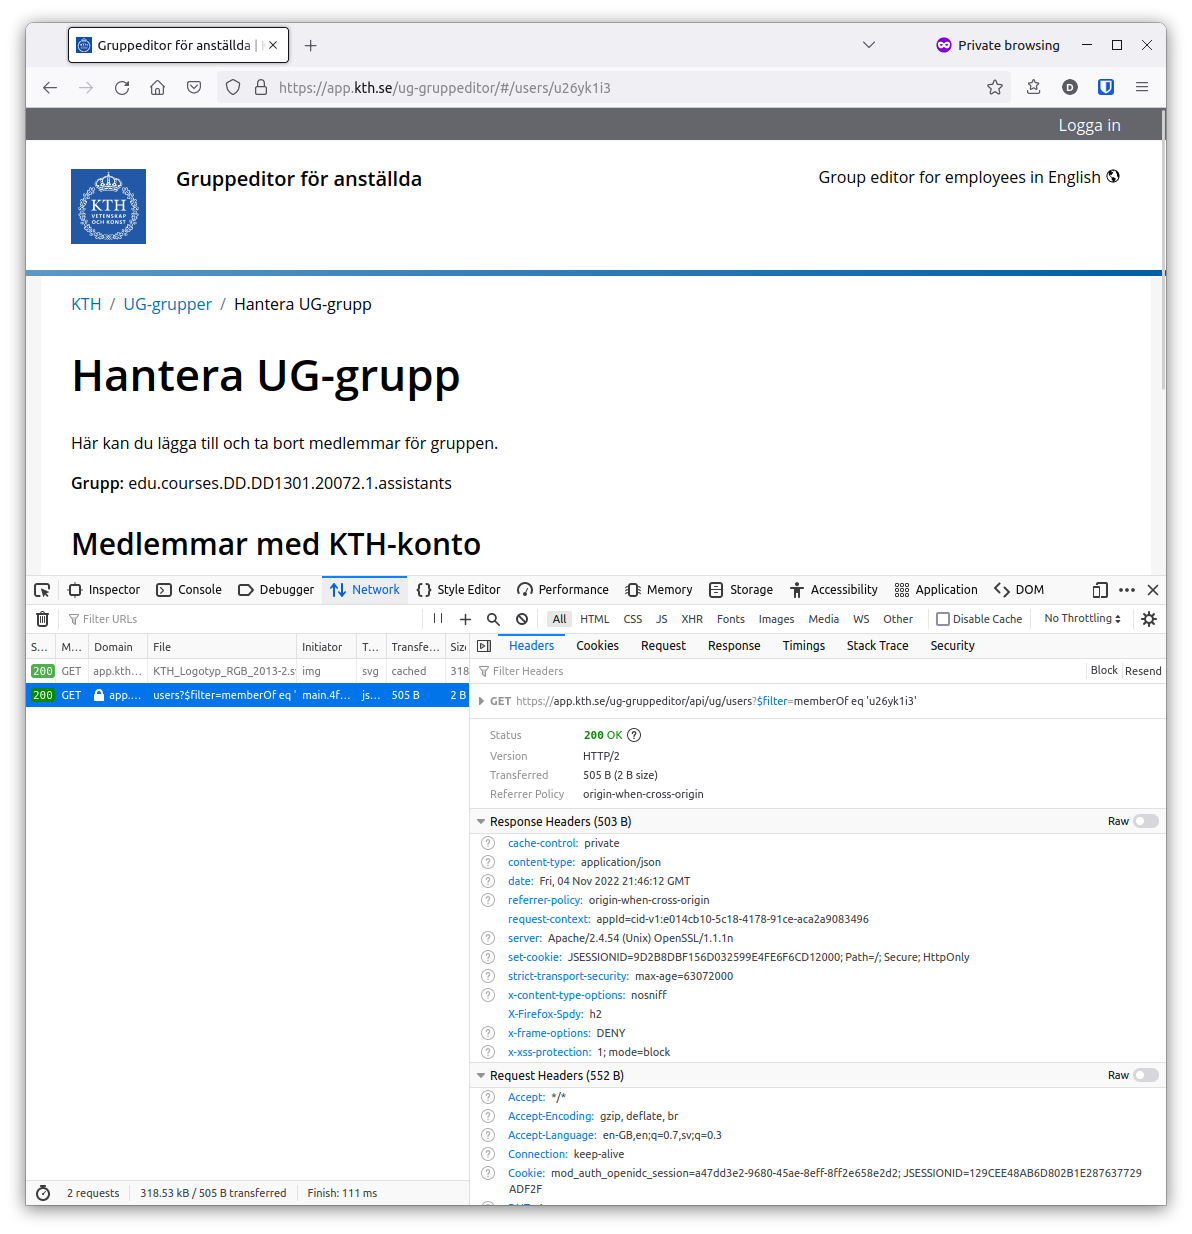
\includegraphics[width=\columnwidth]{figs/ug.png}
  \caption{Screenshot of the KTH UG Editor with Firefox's Developer Tools open, 
  showing network requests made.}
  \label{UGEditor}
\end{figure}

For instance, we can redo the request in \cref{UGEditor} like this:
\begin{minted}{python}
from weblogin.kth import AutologinSession
import os

ug = AutologinSession(os.environ["KTH_LOGIN"],
                      os.environ["KTH_PASSWD"],
                      "https://app.kth.se/ug-gruppeditor/")

response = ug.get("https://app.kth.se/ug-gruppeditor/api/ug/users"
                  "?filter=memberOf eq 'u26yk1i3'")
\end{minted}
The code above will access the API used by the KTH UG group editor service.
It will automatically sign in when needed.
The API URLs don't trigger a redirect to log in, they just give a 401 
unauthorized error.
However, we can use the main URL to the UI to trigger such an event, log in and 
then access the API.
All this happens automatically in the background.

The way we do this is to subclass the \texttt{requests.Session} class to 
intercept all requests of a session to check for signs indicating that we must 
log in.
When we detect such sign, we log in and resume as if nothing ever happened.

\input{../src/weblogin/init.tex}
\input{../src/weblogin/kth.tex}
\input{../src/weblogin/seamlessaccess.tex}

\printbibliography


\end{document}
